% Created 2025-06-08 Sun 18:02
% Intended LaTeX compiler: xelatex
\documentclass[english]{reporti}
\date{}
\title{Reporti: TI-Inspired \LaTeX{} Template.}
\hypersetup{
 pdfauthor={J. L. Benavides},
 pdftitle={Reporti: TI-Inspired \LaTeX{} Template.},
 pdfkeywords={},
 pdfsubject={},
 pdfcreator={Emacs 29.3 (Org mode 9.6.15)}, 
 pdflang={English}}
\begin{document}

\subtitle{LaTeX Template}
\author{Rhyloo - \href{mailto:jorge2@uma.es}{jorge2@uma.es}}
\contact{\href{mailto :jorge2@uma.es}{Feedback about the documentation.}}
\logo{rhyloo_solutions_horizontal.pdf}

\type{README}
\projectcode{REPORTI_DOC_TEMPLATE_v0.0}

\summary{This document pretend to be the documentation of Reporti: A Texas-Instruments inspired LaTeX template.}

\notes{Just copy it and modify under MIT.}

\cover[width=1.35\textwidth][next]

\begin{quote}
[!TIP]

\textbf{TL;DR:} \uline{I recommend you read \texttt{README.pdf}, it is better.}

I had the great idea of use the template for self documentation and I write in org-mode, so maybe the \texttt{RAW} of the \texttt{README.org} is a mesh for you, don't look it.  I recommend you read \texttt{README.pdf}.
\end{quote}

\section{Motivation}
\label{sec:org0a6710a}
At college I read lot of documents about electronics. One of my favorites was \emph{\href{https://e2echina.ti.com/cfs-file/\_\_key/telligent-evolution-components-attachments/00-52-01-00-00-04-59-46/OP-amp-for-everyone.pdf}{Op Amps for everyone}} from Texas Instruments (TI). If you take a moment to analyse the documents in the \texttt{TI\_Examples} folder from this repository, you will agree with me that they are really well done, with great content and a nice design. So, after some time, I found free time to write a \LaTeX{} template. To be honest with you, I don't use \LaTeX{} where I work, and I am not sure if it's used anywhere else, but maybe I or future generations will have to write good nice reports or notes for some crazy school project. :D

So, here is the first version of Reporti, a Texas Instruments-inspired \LaTeX{} template for you all.

\begin{center}
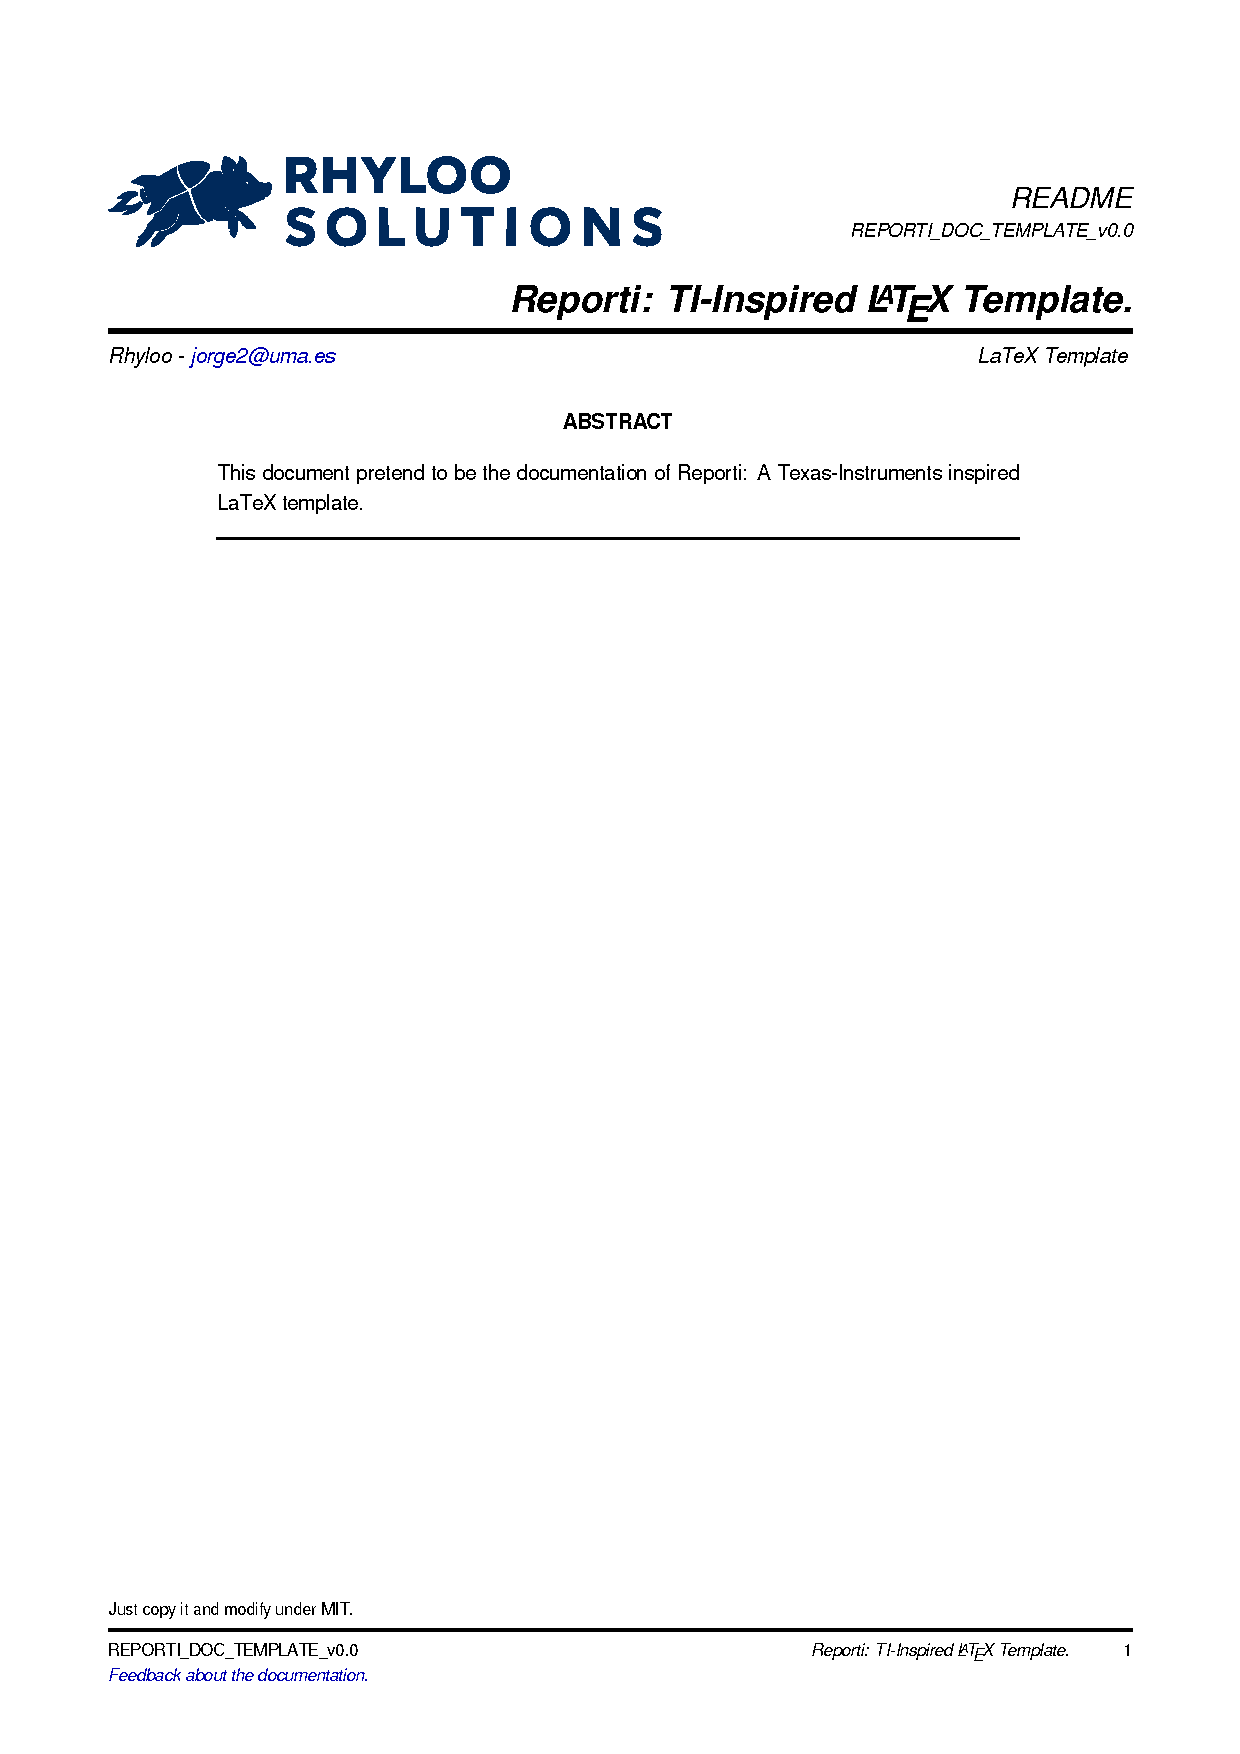
\includegraphics[fbox,height=35em]{./README.pdf}
\end{center}

\section{How to use}
\label{sec:orgebf3ae3}
\subsection{Linux system}
\label{sec:orgb2db262}
Include template on system - If you are planning to use this template with \LaTeX{} with linux download \texttt{reporti.csl} and put it in the path \ldots{}.

\begin{minted}[]{bash}
find -L /home -samefile ./../Reporti/reporti.cls # 
\end{minted}

\emph{home/rhyloo/Documents/\LaTeX{}/Reporti/reporti.cls
/home/rhyloo/texmf/tex/latex/local/reporti.cls
/home/rhyloo}.emacs.d/reporti.cls
/home/rhyloo/snap/languagetool/45/Documents/\LaTeX{}/Reporti/reporti.cls
/home/rhyloo/snap/languagetool/current/Documents/\LaTeX{}/Reporti/reporti.cls
\section{Features}
\label{sec:orgd44179b}
\subsection{Cover page}
\label{sec:org0ab1d51}
Just trying to keep it simple. A .cls file based on report class.

About features, the cover can be customize with the next commands: Check 

\begin{listing}[htbp]
\begin{minted}[]{latex}
\documentclass[draft]{reporti}  %
\cover[width=1.35\textwidth][continue]
\type{Name of doc type}
\code{Project Number/Code} % For more info. Look for naming conventions
\titulo{Project title} 
\autor{Author}
\subtitulo{Subtitle}
\resumen{Summary}
\notes{Some notes in Cover}
\contact{Contact footnote}
\end{minted}
\caption{Control commands for the template}
\end{listing}

\subsection{Table}
\label{sec:org7f12126}
\begin{table}[H]
\caption{Changelog}
\centering
\begin{tabular}{lll}
\hline
Version & Description & Author\\[0pt]
\hline
v0.0 & Initial release & Rhyloo\\[0pt]
\hline
\end{tabular}
\end{table}

\subsection{Images}
\label{sec:org9cf5d28}
\begin{figure}[htbp]
\centering

\includegraphics[fbox,width=.9\linewidth]{./figures/logo/rhyloo_solutions_horizontal.pdf}
\caption{Rhyloo Solutions's logo}
\end{figure}

\section{About images}
\label{sec:orgcbeb805}
The file \texttt{Logo-EII-horizontal.pdf} doesn't have any type of LICENSE on the \href{https://www.uma.es/escuela-de-ingenierias-industriales/info/108566/logo-simbolo-de-la-eii/}{web}. As master's student I can use, maybe you don't, be careful with it.

I am really interested in naming conventions applied to projects. I think is the first part of a good story, I define two names the first is common use and the second is like a code, i.e Fat-Man is the bomb, but if I said Fat-Man-DOC-123HAJK123

Do you have one for owns?? Explain in comments and discuss the best :D

Examples:
\begin{itemize}
\item Texas Instruments have names like: TAS5518-5261K2EVM. According to Deepseek
\begin{itemize}
\item TAS: Indicates a Texas Instruments Audio Solution
\item 5518: The specific model number of the IC.
\item 5261: A code unique to the EVM design
\item K2: Likely denotes a revision or variant of the EVM
\item EVM: Standard suffix for Evaluation Module
\end{itemize}
\end{itemize}

IMO is the first part of a good story like "MarkII" or "Apollo"


\section{About document class}
\label{sec:orga42a8be}

\begin{minted}[]{latex}
\NeedsTeXFormat{LaTeX2e}
\ProvidesClass{reporti}[Template LaTeX based on Texas Instruments note application documentation.]
\LoadClass[10pt, a4paper, twoside]{article}
\end{minted}

\begin{minted}[]{latex}
\DeclareOption{draft}{
    \PassOptionsToPackage{draft}{graphicx}
    \AtEndOfClass{\usepackage{draftwatermark}\SetWatermarkText{DRAFT}}
}

\newcommand{\@mylang}{english}
% Language options
\DeclareOption{spanish}{\renewcommand{\@mylang}{spanish}}
\DeclareOption{english}{\renewcommand{\@mylang}{english}}

\DeclareOption*{\PassOptionsToClass{\CurrentOption}{article}}
\ProcessOptions\relax
\end{minted}

\subsection{Packages}
\label{sec:org978f93b}
I added package geometry becuase I need to config headheight, and page geometry:
\begin{minted}[]{latex}
\RequirePackage{geometry}      % Configuración de márgenes
\setlength{\headheight}{50pt} % 32.05278pt mínimo requerido + margen de seguridad
\geometry{top=3cm, bottom=2.5cm, left=1.83cm, right=1.83cm, footskip=1.2cm}
\end{minted}

Encabezados/pies de página. I defined two styles.
\begin{enumerate}
\item mainstyle: Used for full document elaboration
\item tocstyle: Used by tocs.
\end{enumerate}
\begin{minted}[]{latex}
\RequirePackage{fancyhdr}

\fancypagestyle{mainstyle}{
  \fancyhf{}
  \renewcommand{\headrulewidth}{2pt}
  \renewcommand{\footrulewidth}{1.5pt}
  \ifdefvoid{\@logo}{}{%
    \fancyhead[RE,LO]{\includegraphics[height=2em]{\@logo}\par
      \href{www.rhyloo.com}{www.rhyloo.com}\par\par}
    }
  \fancyhead[LE,RO]{\nouppercase{\rightmark}}
  \fancyfoot[LE]{{\fontsize{8}{35}\selectfont \thepage \hspace{0.8cm} \itshape\@title}}
  \ifdefvoid{\@contact}{\fancyfoot[RE,LO]{{\fontsize{8}{35}\selectfont \ifdefvoid{\@projectcode}{}{\@projectcode}}}}{%
    \fancyfoot[RE,LO]{{\fontsize{8}{35}\selectfont \ifdefvoid{\@projectcode}{}{\@projectcode}\\\itshape\@contact}}
    }
  \fancyfoot[RO]{{\fontsize{8}{35}\selectfont  \itshape\@title \hspace{0.8cm} \thepage}}
}

\fancypagestyle{plain}{
  \fancyhf{}
  \renewcommand{\headrulewidth}{2pt}
  \renewcommand{\footrulewidth}{1.5pt}
  \ifdefvoid{\@logo}{}{%
    \fancyhead[RE,LO]{\includegraphics[height=2em]{\@logo}\par
      \href{www.rhyloo.com}{www.rhyloo.com}\par\par}
    }
  \fancyhead[LE,RO]{\nouppercase{\rightmark}}
  \fancyfoot[LE]{{\fontsize{8}{35}\selectfont \thepage \hspace{0.8cm} \itshape\@title}}
  \ifdefvoid{\@contact}{\fancyfoot[RE,LO]{{\fontsize{8}{35}\selectfont \ifdefvoid{\@projectcode}{}{\@projectcode}}}}{%
    \fancyfoot[RE,LO]{{\fontsize{8}{35}\selectfont \ifdefvoid{\@projectcode}{}{\@projectcode}\\\itshape\@contact}}
    }
  \fancyfoot[RO]{{\fontsize{8}{35}\selectfont  \itshape\@title \hspace{0.8cm} \thepage}}
}

\fancypagestyle{empty}{
  \fancyhf{}
  \renewcommand{\headrulewidth}{2pt}
  \renewcommand{\footrulewidth}{1.5pt}
  \ifdefvoid{\@logo}{}{%
    \fancyhead[RE,LO]{\includegraphics[height=2em]{\@logo}\par
      \href{www.rhyloo.com}{www.rhyloo.com}\par\par}
    }
  \fancyhead[LE,RO]{\nouppercase{\rightmark}}
  \fancyfoot[LE]{{\fontsize{8}{35}\selectfont \thepage \hspace{0.8cm} \itshape\@title}}
  \ifdefvoid{\@contact}{\fancyfoot[RE,LO]{{\fontsize{8}{35}\selectfont \ifdefvoid{\@projectcode}{}{\@projectcode}}}}{%
    \fancyfoot[RE,LO]{{\fontsize{8}{35}\selectfont \ifdefvoid{\@projectcode}{}{\@projectcode}\\\itshape\@contact}}
    }
  \fancyfoot[RO]{{\fontsize{8}{35}\selectfont  \itshape\@title \hspace{0.8cm} \thepage}}
}

\fancypagestyle{tocstyle}{
  \fancyhf{}
  \renewcommand{\headrulewidth}{2pt}
  \renewcommand{\footrulewidth}{1.5pt}
  \ifdefvoid{\@logo}{}{%
    \fancyhead[RE,LO]{\includegraphics[height=2em]{\@logo}\par
      \href{www.rhyloo.com}{www.rhyloo.com}\par\par}
  }
  \fancyhead[LE,RO]{}
  \fancyfoot[LE]{{\fontsize{8}{35}\selectfont \thepage \hspace{0.8cm} \itshape\@title}}
  \ifdefvoid{\@contact}{\fancyfoot[RE,LO]{{\fontsize{8}{35}\selectfont \ifdefvoid{\@projectcode}{}{\@projectcode}}}}{%
    \fancyfoot[RE,LO]{{\fontsize{8}{35}\selectfont \ifdefvoid{\@projectcode}{}{\@projectcode}\\\itshape\@contact}}
  }
  \fancyfoot[RO]{{\fontsize{8}{35}\selectfont  \itshape\@title \hspace{0.8cm} \thepage}}
}

\fancypagestyle{titlepagestyle}{
  \fancyhf{}
  \renewcommand{\headrulewidth}{0pt}
  \renewcommand{\footrulewidth}{1.5pt}
  \fancyfoot[LE]{{\fontsize{8}{35}\selectfont \thepage \hspace{0.8cm} \itshape\@title}}
  \ifdefvoid{\@contact}{  \fancyfoot[RE,LO]{{\fontsize{8}{35}\selectfont \ifdefvoid{\@projectcode}{}{\@projectcode}}}}{
  \fancyfoot[RE,LO]{{\fontsize{8}{35}\selectfont \ifdefvoid{\@projectcode}{}{\@projectcode}\\\itshape\@contact}}}
  \fancyfoot[RO]{{\fontsize{8}{35}\selectfont  \itshape\@title \hspace{0.8cm} \normalfont\thepage}}
}
\end{minted}

\begin{minted}[]{latex}
\RequirePackage{xparse}        % Para comandos avanzados
\end{minted}

\begin{minted}[]{latex}

\RequirePackage{xcolor}        % Manejo de colores
\RequirePackage{titlesec}      % Estilos de secciones
\RequirePackage{graphicx}      % Manejo de imágenes

% Default: English

\RequirePackage[\@mylang]{babel}


\RequirePackage{hyperref}      % Hipervínculos
\hypersetup{
    colorlinks = true,
    linkcolor = blue!70!black,
    urlcolor = blue!70!black,
    citecolor = green!60!black
}


\RequirePackage{fontspec}      % Fuentes modernas
\setmainfont{FreeSans}


\RequirePackage[export]{adjustbox}
\RequirePackage{datetime2}     % Manejo de fechas profesional

\RequirePackage{etoolbox}      % Utilidades de macros
\RequirePackage{tabularx}
\RequirePackage{float}
\RequirePackage{booktabs}
\RequirePackage{multirow}
\RequirePackage{tocloft}
\RequirePackage[tableposition=above]{caption}
\RequirePackage[figure,table,listing]{totalcount}
\RequirePackage{xstring} % Add near the top of the file
\RequirePackage{underscore}
\RequirePackage{longtable}
\RequirePackage{wrapfig}
\RequirePackage{rotating}
\RequirePackage[normalem]{ulem}
\RequirePackage{amsmath}
\RequirePackage{amssymb}
\RequirePackage{capt-of}


\RequirePackage[newfloat,outputdir=./build]{minted}
\usemintedstyle{emacs}
\RequirePackage{caption}

\newcommand{\test}{Code}

\SetupFloatingEnvironment{listing}{%
  name={\test}}
\renewcommand{\thelisting}{\arabic{section}-\arabic{listing}}




\RequirePackage[most]{tcolorbox}
% Configuración de datetime2 para español
\DTMsetup{useregional=numeric}

\graphicspath{{figures/}{figures/logo/}}
\end{minted}

\subsection{Doument Commands}
\label{sec:org578908b}
\begin{minted}[]{latex}
\newcommand{\@metadata}{} % Registro de metadatos

\NewDocumentCommand{\autor}{m}{%
    \def\@autor{#1}%
    \listadd{\@metadata}{Autor: #1}%
}
\NewDocumentCommand{\fecha}{O{\DTMtoday}}{%
    \def\@fecha{#1}%
    \listadd{\@metadata}{Fecha: #1}%
}
\NewDocumentCommand{\summary}{m}{%
    \def\@summary{#1}%
    \ifx\@summary\@empty\else
        \gappto\@afterabstract{\@printsummary}%
    \fi
}
\NewDocumentCommand{\subtitle}{m}{%
    \def\@subtitle{#1}%
    \listadd{\@metadata}{Subtítulo: #1}%  % Opcional: para mostrar en metadata
}
\NewDocumentCommand{\type}{m}{%
    \def\@type{#1}%
    \listadd{\@metadata}{Type: #1}%  % Opcional: para mostrar en metadata
}

\NewDocumentCommand{\projectcode}{m}{%
    \def\@projectcode{#1}%
    \listadd{\@metadata}{Projectcode: #1}%  % Opcional: para mostrar en metadata
}
\NewDocumentCommand{\notes}{m}{%
    \def\@notes{#1}%
    \listadd{\@metadata}{Notes: #1}%  % Opcional: para mostrar en metadata
}
\NewDocumentCommand{\contact}{m}{%
    \def\@contact{#1}%
    \listadd{\@metadata}{Contact: #1}%  % Opcional: para mostrar en metadata
}
\NewDocumentCommand{\toc}{m}{%
    \def\@toc{#1}%
    \listadd{\@metadata}{TOC: #1}%  % Opcional: para mostrar en metadata
}
\NewDocumentCommand{\logo}{m}{%
    \def\@logo{#1}%
    \listadd{\@metadata}{LOGO: #1}%  % Opcional: para mostrar en metadata
}


\renewcommand{\sectionmark}[1]{\markright{#1}}
\renewcommand{\subsectionmark}[1]{} % Subsecciones no modifican los headers


% ========================
% 4. Estilos de Títulos
% ========================
\setlength{\voffset}{10pt} % Ajusta según necesidad para evitar warnings
\setlength{\headsep}{5pt} % Ajusta según necesidad para evitar warnings

% Definir formato de títulos
\titleformat{\section}
  {\large\bfseries} % Formato del texto
  {\thesection.\hspace{2em}}   % Etiqueta: Número + 4em de espacio
  {0pt}                        % Separación entre etiqueta y título
  {}                           % Código antes del título

\titleformat{\subsection}
  {\large\itshape\bfseries}
  {\thesubsection.\hspace{1.25em}} % 3em de espacio
  {0pt}
  {}

\titleformat{\subsubsection}
  {\bfseries}
  {\hspace{3.5em}} % 2em de espacio
  {0pt}
  {}

% Ajustar espaciado vertical (opcional)
\titlespacing{\section}{0pt}{12pt}{6pt}
\titlespacing{\subsection}{0pt}{12pt}{6pt}
\titlespacing{\subsubsection}{0pt}{12pt}{6pt}

\newlength{\originalparskip}
% ========================
% 6. Cover
% ========================
\NewDocumentCommand{\cover}{
  O{width=0.8\textwidth}  % #1 = width spec (default 0.8\textwidth)
  O{}                     % #2 = “continue” flag (default empty)
}{%
  \begingroup % Grupo local para cambios de espaciado
  \pagestyle{tocstyle} %
  \setlength{\originalparskip}{\parskip} %
  \renewcommand{\baselinestretch}{0.4}%
  \renewcommand{\parskip}{\originalparskip}%
  \begin{titlepage}
    \thispagestyle{titlepagestyle}
    % —– HEADER WITH LOGO & INSTITUTIONAL DATA —–
    \ifdefvoid{\@logo}{\vspace*{2em}}{
    \noindent\begin{minipage}[t]{0.4\textwidth}
    \includegraphics[#1]{\@logo}
    \end{minipage}%
    }
    \hfill    
    \begin{minipage}[t]{0.6\textwidth}
      \vspace{-2\baselineskip}
      \raggedleft
      \ifdef{\@type}{\fontsize{14}{35}\selectfont\itshape\@type}{}\par
      \ifdef{\@projectcode}{\fontsize{9}{35}\selectfont\itshape\@projectcode}{}
    \end{minipage}
    
    \vspace{0.5\baselineskip} 

    % —– TITLE —–
    \begin{flushright}
      {\fontsize{18}{35}\selectfont\bfseries\itshape\@title}
    \end{flushright}
    \vspace*{-1\baselineskip} 
    \rule{\textwidth}{2pt}

    % —– AUTHOR & SUBTITLE —–
    \noindent\begin{minipage}{0.7\textwidth}
    \raggedright
    \ifdef{\@author}{{\fontsize{10}{35}\selectfont\itshape\@author}}{}
    \end{minipage}
    \hfill
    \begin{minipage}{0.25\textwidth}
      \raggedleft
      \ifdef{\@subtitle}{{\fontsize{10}{35}\selectfont\itshape\@subtitle}}{}
    \end{minipage}

    % —– ABSTRACT (IF ANY) —–
    \ifdefvoid{\@summary}{}{%
      \vspace{0.75cm}
      
      \hspace{1.75cm}
      \begin{minipage}{13.6cm}
        \begin{center}
          \noindent{\bfseries ABSTRACT}
        \end{center}
            {\fontsize{10}{35}\selectfont\@summary}\par
            \rule{\textwidth}{1pt}
      \end{minipage}
    }
    % —– EITHER “CONTINUE” CASE OR DEFAULT NOTES —–
    \ifstrequal{#2}{continue}{
      % ==== continue: TOC + lists *inside* the titlepage ====
      \tocloftpagestyle{titlepagestyle}
      
      \hspace{1.75cm}
      \begin{minipage}{13.6cm}
        {\fontsize{9}{35}\selectfont
          \tableofcontents
          \iftotalfigures   \listoffigures  \fi
          \iftotaltables    \listoftables   \fi
          \iftotallistings  \listoflistings \fi
        }
    \end{minipage}}{}
    \vfill
    \ifdefvoid{\@notes}{}{%
      \noindent\raggedright{\fontsize{8}{35}\selectfont\@notes\vspace{-1\baselineskip}}}
  \end{titlepage}

    % —– EITHER “CONTINUE” CASE OR DEFAULT NOTES —–
  \endgroup
  
  \ifstrequal{#2}{continue}{}{
    \tocloftpagestyle{tocstyle}
    \pagestyle{tocstyle}
    \thispagestyle{tocstyle}
    \tableofcontents
    \pagestyle{tocstyle}
    \thispagestyle{tocstyle}    
    \iftotalfigures   \listoffigures  \fi
        \pagestyle{tocstyle}
    \thispagestyle{tocstyle}
    \iftotaltables    \listoftables   \fi
        \pagestyle{tocstyle}
    \thispagestyle{tocstyle}
    \iftotallistings    \listoflistings \fi
    \markright{}     % Limpiar explícitamente rightmark
    }

  \clearpage
  %% \markboth{}{}   % Limpiar leftmark y rightmark
  \pagestyle{mainstyle}
}

\AddToHook{cmd/section/before}{%
  \clearpage
}


\setlength{\cftbeforesecskip}{0pt}
\renewcommand{\cftsecleader}{\cftdotfill{\cftdotsep}}
\renewcommand{\cftdotsep}{1}% Default is 4.5

\renewcommand{\cftaftertoctitleskip}{2em}
\renewcommand{\cftafterloftitleskip}{2em}
\renewcommand{\cftafterlottitleskip}{2em}

\renewcommand{\cftfigindent}{0pt}
\renewcommand{\cftfigpresnum}{\figurename~}
\renewcommand{\cftfigaftersnum}{.}
\setlength{\cftfignumwidth}{5em}
\renewcommand{\thefigure}{\arabic{section}-\arabic{figure}}
\renewcommand{\cftsecpagefont}{\normalsize}


% =============================================
% List of Tables Customization
% =============================================
% 1. Set table numbering format: section-table (e.g., 1-1)
\renewcommand{\thetable}{\arabic{section}-\arabic{table}}

% 2. Configure table entries in List of Tables
\renewcommand{\cfttabindent}{0pt}               % Remove indentation
\renewcommand{\cfttabpresnum}{\tablename~}      % Prefix: "Table "
\renewcommand{\cfttabaftersnum}{.}              % Suffix: "."
\setlength{\cfttabnumwidth}{5em}                % Width for table numbers

% 3. (Optional) Set section page numbers in TOC
\renewcommand{\cftsecpagefont}{\normalsize}     % Normal font for section page numbers




\setlength{\parindent}{0pt}
\setlength{\baselineskip}{50pt}
\renewcommand{\baselinestretch}{1.2} % Ajuste principal (20% más de espacio)


\makeatletter
\apptocmd{\@afterheading}{
  \vspace{-0.5\baselineskip}
  \setlength{\parskip}{12pt}
  }{}{}
\makeatother



\addto\captionsspanish{%
  \renewcommand{\contentsname}{\hfill\bfseries\normalsize Contenido\hfill}
  \renewcommand{\figurename}{Figura} % Override figure name globally
  \renewcommand{\tablename}{Tabla}
  \renewcommand{\test}{Código}
\renewcommand{\listfigurename}{\hfill\bfseries\normalsize Lista de figuras\hfill}
\renewcommand{\listtablename}{\hfill\bfseries\normalsize Lista de tablas\hfill}
\renewcommand{\listlistingname}{\hfill\bfseries\normalsize Lista de códigos\hfill}
}

\addto\captionsenglish{%
  \renewcommand{\contentsname}{\hfill\bfseries\normalsize Content\hfill}
  \renewcommand{\tablename}{Table}
  \renewcommand{\figurename}{Figure} % Override figure name globally
  \renewcommand{\test}{Code}
\renewcommand{\listfigurename}{\hfill\bfseries\normalsize List of figures\hfill}
\renewcommand{\listtablename}{\hfill\bfseries\normalsize List of tables\hfill}
\renewcommand{\listlistingname}{\hfill\bfseries\normalsize List of codes\hfill}
}

\makeatletter
\renewcommand{\l@listing}[2]{%
  \renewcommand{\figurename}{\test} % Override figure name globally
  \l@figure{#1}{#2}%
}
\makeatother

\tocloftpagestyle{tocstyle}
\end{minted}
\section{Known - Bugs}
\label{sec:orgde85a39}
\subsection{{\bfseries\sffamily TODO} If there more than X sections the template do crazy things.}
\label{sec:org2737276}
\subsection{{\bfseries\sffamily TODO} Change langs is not easy as I want.}
\label{sec:orga5c0f5d}
\subsection{{\bfseries\sffamily TODO} Adjust toc style not in header}
\label{sec:org5008756}
\subsection{{\bfseries\sffamily TODO} Modificar la web del header}
\label{sec:org47ed2ce}
\end{document}
